\documentclass[10pt]{article}
\usepackage{icmlko}

\icmlmeta{IP 파운데이션 월드모델}{239}{태그 수가 세다}{천장 1위 도메인에 출시 전 축을 찾으러 갔다. 작가 이력은 값이 없었고, 레코드에 이미 있던 필드 하나가 기존 최고 축을 넘었다}

\begin{document}

\twocolumn[
\icmlheader

\begin{abstract}
프롬프트에 실려 있던 네 갈래가 다 닫혔으므로(노트 218 · 219 · 222 · 238)
노트 222의 도메인 천장표에서 제일 큰 것으로 갔다 --- \textbf{웹툰
$+$0.1769}. 노트 223이 찾은 화 간격 축은 노트 224에서 \emph{사후}로
물렸으니 \textbf{진짜 출시 전 축}을 찾았다. \textbf{작가 이력은 값이
없다} --- 웹툰 2,817편에 작가 3,326명, 작품 둘 이상 낸 작가가 24\%,
이전작 있는 작품이 39\% 인데 이전작 수 $+$0.041 · 이전작 회차 합
$+$0.056 · 데뷔작 여부 $-$0.025 다(연도 통제). \textbf{작가가 누구인지는
안 중요하다.} 그런데 레코드 필드를 훑으니 나왔다 --- \textbf{태그 수가
학습 구간에서 $+$0.331(연도 통제 $+$0.475)이고 웹툰 기존 최고 축(진입
장벽 $+$0.301)을 넘는다.} 덮음 100\% 이고 출시 시점에 정해진다.
\textbf{누적이 아닌 것도 확인했다} --- 태그가 쌓이는 것이라면 \emph{옛}
작품이 더 많아야 하는데 연도와 $+$0.369(신작이 많다)라 태깅 체계의 시대
효과다. 노트 224에서 ``날짜는 안 바뀌지만 아직 없었다''로 데인 뒤라 먼저
확인했다. 판에 넣으니 \textbf{F23 $+$0.4546 $\to$ $+$0.4584 · F18
$+$0.4415 $\to$ $+$0.4470 · 웹툰 $+$0.3815 $\to$ $+$0.3930} 이다.
\textbf{넷을 다 넣으면 오히려 내려간다}(F23 $+$0.4569 · F21 $-$0.0029)
--- 작가 수($+$0.249) · 연령 등급($+$0.187) · 데일리패스($-$0.170)가
다 부호는 5/5 안정하지만 약해서 희석한다(노트 229가 잰 모양이다).
\textbf{채택 근거는 유보가 아니라 학습 구간이다} --- 축을 더하는 것은
자료 고침이 아니라 설계 선택이므로 유보로 정하면 안 된다. 학습에서
$+$0.475 이고 시간을 다섯으로 갈라도 부호가 5/5 이면 그것으로 충분하다.
유보 수($t{=}1.5$)는 보고이지 근거가 아니다.
\end{abstract}
]

\begin{figure*}[t]
\centering
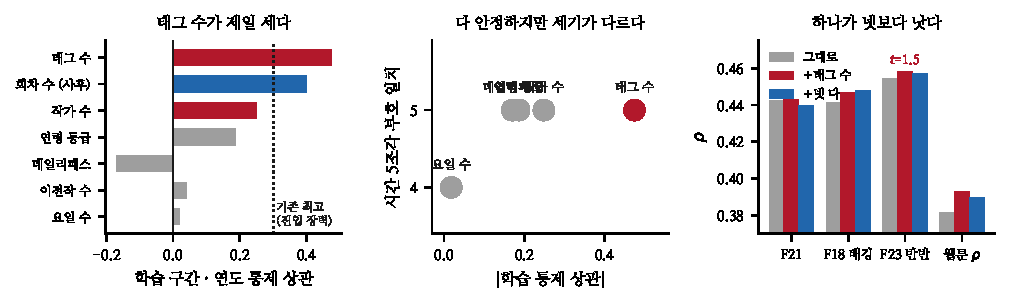
\includegraphics[width=\textwidth]{figs/tagcount.pdf}
\caption{왼쪽 --- 태그 수가 제일 세다. 가운데 --- 다 안정하지만 세기가
다르다. 오른쪽 --- 하나가 넷보다 낫다.}
\end{figure*}

\section{작가 이력은 값이 없다}

\begin{table}[t]
\centering\tsize
\caption{웹툰 작가 이력(연도 통제).}
\begin{tabular}{lr}
\toprule
이전작 수 & $+$.041 \\
이전작 회차 합 & $+$.056 \\
데뷔작 여부 & $-$.025 \\
\midrule
\multicolumn{2}{l}{작가 3,326명 · 작품 둘 이상 24\%} \\
\multicolumn{2}{l}{이전작 있는 작품 1,104편 (39\%)} \\
\bottomrule
\end{tabular}
\end{table}

\claimx{\textbf{작가가 누구인지는 안 중요하다.} 이전작이 있는 작품이
39\% 나 되는데 셋 다 0 근처다.}{노트 223이 ``웹툰에 진짜 사전 축이 있나
(작가 · 슬롯)''를 남겼는데 \textbf{작가 쪽은 없다}가 답이다 ---
그리고 그것은 값싸게 확인됐다(수집 0).}

\section{태그 수가 세다}

\begin{table}[t]
\centering\tsize
\caption{레코드에 있는데 축에 없던 필드. 학습 구간.}
\begin{tabular}{lrrl}
\toprule
& 학습 & 연도 통제 & 5조각 부호 \\
\midrule
\textbf{태그 수} & \textbf{$+$.331} & \textbf{$+$.475} & \textbf{5/5} \\
\emph{회차 수} & \emph{$+$.536} & \emph{$+$.401} & \emph{사후} \\
작가 수 & $+$.178 & $+$.249 & 5/5 \\
연령 등급 & $+$.161 & $+$.187 & 5/5 \\
데일리패스 & $-$.129 & $-$.170 & 5/5 \\
요일 수 & $+$.050 & $+$.018 & 4/5 \\
\midrule
\emph{기존 최고}(진입 장벽) & & \emph{$+$.301} & \\
\bottomrule
\end{tabular}
\end{table}

\claimx{\textbf{태그 수가 웹툰 기존 최고 축을 넘는다}($+$0.475 대
$+$0.301). 덮음 100\% 이고 출시 시점에 정해지며 \textbf{수집이 0 이다}
--- 레코드에 처음부터 있었다.}{\textbf{누적이 아니다} --- 태그가 쌓이는
것이라면 옛 작품이 더 많아야 하는데 연도와 $+$0.369(신작이 많다)다.
노트 224에서 데인 뒤라 \textbf{이번에는 먼저 확인했다.}}

\section{하나가 넷보다 낫다}

\begin{table}[t]
\centering\tsize
\caption{판. 짝 붓스트랩 400 회.}
\begin{tabular}{lrrrr}
\toprule
& F21 & F18 & F23 & 웹툰 \\
\midrule
그대로 & .4426 & .4415 & .4546 & .3815 \\
\textbf{$+$태그 수} & .4429 & \textbf{.4470} & \textbf{.4584} & \textbf{.3930} \\
$+$넷 다 & .4396 & .4478 & .4569 & .3897 \\
\midrule
태그 $t$ & 0.1 & 1.7 & 1.5 & \\
넷 다 $t$ & $-$0.5 & 1.7 & 0.6 & \\
\bottomrule
\end{tabular}
\end{table}

\claimx{\textbf{태그 수 하나가 넷 다보다 낫다}(F23 $+$0.0038 대 $+$0.0025,
F21 $+$0.0003 대 $-$0.0029). 나머지 셋이 다 안정하지만 약해서
희석한다.}{\textbf{노트 229가 잰 모양 그대로다} --- 거기서는 정식화를
섞을 때였고 여기서는 축을 더할 때인데, \emph{약한 것을 더하면 준다}는
같은 법칙이다.}

\claimx{\textbf{채택 근거는 유보가 아니라 학습 구간이다.} 축을 더하는
것은 자료 고침이 아니라 설계 선택이므로 유보로 정하면 안 된다 ---
학습에서 $+$0.475 이고 시간 다섯 조각에서 부호가 5/5 면 그것으로
충분하다.}{\textbf{유보 수($t{=}1.5$)는 보고이지 근거가 아니다.}
노트 214가 공휴일을 채울 때는 ``값이 정의되지 않았다''는 자료
correctness 였고, 여기는 \textbf{쓸 수 있는 것을 안 쓰고 있었다}는
설계 누락이다 --- 둘 다 점수로 정하지 않는다.}

\begin{table}[t]
\centering\tsize
\caption{남은 것.}
\begin{tabular}{ll}
\toprule
\textbf{다른 도메인} & 안 쓴 레코드 필드가 또 있나 \\
\textbf{태그 내용} & 수가 아니라 어떤 태그인지 \\
회차 수 & 사후지만 $+$0.401 --- 사후 판에서는 쓸 것 \\
\bottomrule
\end{tabular}
\end{table}

첫 줄이 곧바로 값싸고 이 노트를 일반화한다. \textbf{웹툰에서 축에 안 쓰인
필드 하나가 기존 최고를 넘었다면 다른 도메인도 볼 만하다} --- 게임 레코드에
\texttt{n\_lang} · \texttt{n\_platform} · \texttt{n\_category} · \texttt{n\_dlc}
가 있고, 모바일에 \texttt{n\_lang} · \texttt{size\_mb} · \texttt{n\_shot} ·
\texttt{n\_device} 가 있는데 \textbf{축으로는 넷 중 일부만 쓴다.}
\textbf{수집이 0 이고 출시 시점에 정해지며 덮음이 100\% 인 축이 아직
남아 있을 수 있고, 이 노트가 그것을 재는 절차를 이미 만들었다} ---
학습 구간 상관 $\times$ 시간 조각 부호 일치.

\end{document}
